%%%%%%%%%%%% PACKAGES %%%%%%%%%%%%
\documentclass{template}
\usepackage{graphicx,parskip,appendix,float}
\usepackage{tikz,pgfplots}
\usepackage{subcaption}
\usepackage{multirow}
\pgfplotsset{compat=1.18}
\usetikzlibrary{shapes.geometric, arrows.meta, positioning, calc}
\usepackage[ruled]{algorithm2e}
\usepackage{url,amsmath,amssymb,fancybox,listings,pdfpages,caption,multicol,datetime,rotating,booktabs}
\usepackage{csquotes}

%%%%%%%%%%%% LAYOUT %%%%%%%%%%%%
\usepackage[a4paper, margin=2.2cm]{geometry}
\setstretch{1.15}
\renewcommand{\thesection}{\arabic{section}}
\renewcommand{\thetable}{\arabic{table}}
\renewcommand{\thefigure}{\arabic{figure}}
\renewcommand{\theequation}{\arabic{equation}}
\usepackage{titlesec}
\titlespacing*{\section}{0pt}{1.1em}{0.6em}
\titlespacing*{\subsection}{0pt}{0.9em}{0.45em}
\setlength{\textfloatsep}{10pt plus 2pt minus 2pt}
\setlength{\intextsep}{10pt plus 2pt minus 2pt}
\captionsetup{font=small, skip=5pt}

%%%%%%%%%%%% REFERENCES %%%%%%%%%%%%
\usepackage[style=authoryear,giveninits,uniquename=init,backend=biber]{biblatex}
\addbibresource{thesis.bib}

%%%%%%%%%%%% HYPERREF (load last) %%%%%%%%%%%%
\usepackage[pagebackref=false,pdffitwindow=true]{hyperref}
\hypersetup{
    pdftitle    = {Impact of Weather Variables on Short-Term Electricity Demand Forecasting in Singapore: A Comparative Study with PPSO-Optimised Models},
    pdfauthor   = {Amanda An, Ryaan Le, Nolen Dao, Louise Nguyen, Kain Tran, Uri Duong},
    pdfsubject  = {Electricity Demand Forecasting, Machine Learning},
    pdfkeywords = {electricity demand, forecasting, CatBoost, PPSO, Singapore, weather},
    colorlinks  = true, anchorcolor = blue, filecolor = blue, urlcolor = blue,
    linkcolor   = blue,
    citecolor   = blue,
}

%%%%%%%%%%%% COLOURS & MISC %%%%%%%%%%%%
\definecolor{colBackGrnd}{rgb}{1,1,0.8}
\definecolor{colIdentifier}{rgb}{0,0,0}
\definecolor{colComments}{rgb}{0,.5,0}
\definecolor{colWhite}{rgb}{1,1,1}

\newcommand{\MyHookSign}{\hbox{\ensuremath\hookleftarrow}}

\lstset{%
    float=H,
    basicstyle=\ttfamily\footnotesize,
    identifierstyle=\color{colIdentifier},
    keywordstyle=\color{colIdentifier},
    stringstyle=\color{colIdentifier},
    commentstyle=\color{colIdentifier},
    columns=flexible,
    tabsize=2,
    frame=single,
    extendedchars=true,
    showspaces=false,
    showstringspaces=false,
    numbers=left,
    numberstyle=\footnotesize,
    breaklines=true,
    prebreak={\space\MyHookSign},
    language=Java,
    backgroundcolor=\color{colBackGrnd},
    breakautoindent=true,
    captionpos=b
}

\sloppy

%%%%%%%%%% DOCUMENT %%%%%%%%%%%%
\begin{document}

\DeclareGraphicsExtensions{.jpg,.png,.gif,.pdf}

\title{\huge{Impact of Weather Variables on Short-Term Electricity Demand Forecasting in Singapore: A Comparative Study with PPSO-Optimised Models}}
\author{Amanda An \\ Ryaan Le \\ Nolen Dao \\ Louise Nguyen \\ Kain Tran \\ Uri Duong}
\rpttype{Degree}
\principaladviser{Dr. Young Lee}

%%%%%%%%%%%% ACKNOWLEDGEMENTS (replaces Declaration page) %%%%%%%%%%%%
\makeatletter
\def\declpage{%
\prefacesection{Acknowledgements}
    We would like to thank Dr.\ Young Lee for his guidance, constructive
    feedback throughout this project. We also thank the
    Singapore Energy Market Authority (EMA) for making electricity demand
    data publicly available, and the open-source communities behind
    scikit-learn, XGBoost, CatBoost, and the Open-Meteo weather API,
    whose tools made this work possible.
\vfill}
\makeatother

\beforeabstract
\afterabstract

\section{Introduction}\label{sec:intro}
\pagenumbering{arabic} \setcounter{page}{1}

Singapore's power grid serves roughly 5.9 million residents in a tropical climate where air-conditioning runs year-round; national electricity consumption exceeded 55\,TWh in 2024 \parencite{ema2025statistics}. Because cooling is the single largest end-use in buildings, even small shifts in temperature or humidity can noticeably swing demand \parencite{zhao2012review}, and holidays, weekends, and monsoon transitions add further irregularity. For grid operators, getting short-term forecasts right is not optional---it directly affects generation scheduling and system reliability.

Classical approaches like ARIMA and exponential smoothing assume linear, stationary dynamics and tend to fall short once non-linear weather--demand interactions come into play \parencite{almusaylh2018forecasting}. Tree-based machine learning models handle these interactions much better, but their performance depends heavily on hyperparameter choices, and manual tuning is both tedious and often sub-optimal. Zhang et al.\ \parencite{zhang2023catboostppso} demonstrated that pairing CatBoost with Phasor Particle Swarm Optimisation (PPSO) beats five other meta-heuristics---however, their experiment used hourly data from a \emph{single residential customer} and only tuned the favoured model. Two questions naturally follow: does the approach still work at the scale of \emph{daily national-level} demand in a tropical climate, and does CatBoost-PPSO retain its edge when \emph{every} competing model is given the same tuning budget?

We address both questions. Specifically, we (i) construct a daily Singapore dataset by merging EMA demand records with Open-Meteo weather data (February 2023 -- December 2025); (ii) engineer 16 features spanning weather, derived-comfort, calendar, and autoregressive categories; (iii) compare eight model configurations---a Lag-1 baseline, Linear Regression, Random Forest, XGBoost, and CatBoost, plus PPSO-tuned variants of each tree model under an \emph{identical} budget---across six evaluation metrics; and (iv) deploy the best model through a web portal (FastAPI + React) aimed at non-technical users. Intra-day resolution, sector-level decomposition, and deep learning architectures are left for future work.

\section{Related Work}\label{sec:related}

Classical time-series methods such as ARIMA and Holt-Winters handle linear temporal patterns reasonably well, but they consistently lose to machine learning once exogenous weather variables enter the picture. Almusaylh et al.\ \parencite{almusaylh2018forecasting} showed that SVR and MARS outperform ARIMA on short-term Australian demand, and Schirmer et al.\ \parencite{schirmer2019evaluation} found tree-based models clearly superior to linear regression for residential load prediction. Within the tree-ensemble family, Random Forest \parencite{breiman2001randomforest} controls variance via bagging; XGBoost \parencite{chen2016xgboost} introduces regularised sequential boosting and has become a go-to model in energy forecasting \parencite{khan2020hybrid}; and CatBoost \parencite{prokhorenkova2018catboost} offers ordered boosting with native categorical support---a useful property for demand data that includes day-of-week, month, and holiday flags. Weather, holidays, and weekends are well-established demand drivers \parencite{khan2021influencing}.

On the tuning side, meta-heuristic optimisation can make a substantial difference---Li et al.\ \parencite{li2020datadrivenstrategy} reported a 42\% accuracy gain from PSO-tuned models on university building data. PPSO \parencite{ghasemi2019ppso} is a variant of PSO that uses a phase angle to modulate the cognitive and social velocity components through periodic functions, which removes the need to hand-tune inertia and acceleration coefficients. Zhang et al.\ \parencite{zhang2023catboostppso} applied CatBoost-PPSO to hourly consumption of a single residential customer and found it outperformed five alternative meta-heuristics.

However, there is a methodological concern in prior work: tuning is typically applied only to the authors' preferred model, so it is unclear whether the reported advantage comes from the algorithm itself or simply from having better hyperparameters. Additionally, CatBoost-PPSO has not been tested on daily national-level demand in a tropical climate. Our project tackles both of these gaps.

\section{Methodology}\label{sec:method}

\subsection{Pipeline Overview}

Our system follows a modular, end-to-end pipeline (Figure~\ref{fig:pipeline_flowchart}) controlled by a single YAML configuration file. It covers data acquisition, feature engineering, a chronological train/test split, model training with optional PPSO tuning, and multi-metric evaluation. Each stage is implemented as a standalone Python module, making it straightforward to swap components or rerun individual steps.

\begin{figure}[H]
\centering
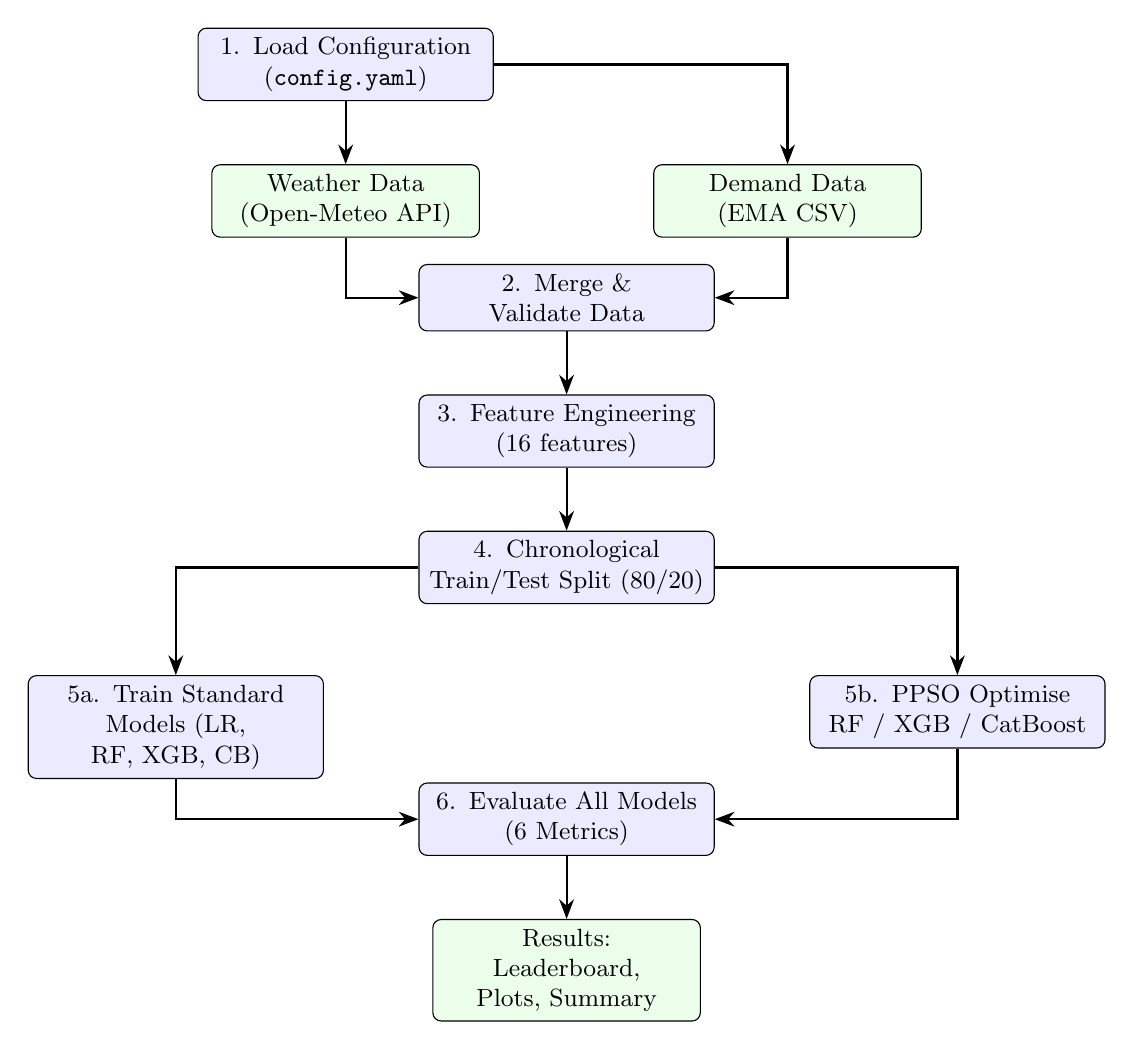
\begin{tikzpicture}[
    node distance=0.8cm and 1.2cm,
    block/.style={rectangle, draw, fill=blue!8, text width=10em, text centered, minimum height=2.4em, rounded corners=3pt, font=\small},
    data/.style={rectangle, draw, fill=green!8, text width=9em, text centered, minimum height=2.2em, rounded corners=3pt, font=\small},
    arrow/.style={-{Stealth[length=2.5mm]}, thick}
]
\node[block] (config) {1. Load Configuration\\(\texttt{config.yaml})};
\node[data, below=of config] (weather) {Weather Data\\(Open-Meteo API)};
\node[data, right=2.2cm of weather] (demand) {Demand Data\\(EMA CSV)};
\node[block, below=0.8cm of $(weather)!0.5!(demand)$] (merge) {2. Merge \& Validate Data};
\node[block, below=of merge] (preprocess) {3. Feature Engineering\\(16 features)};
\node[block, below=of preprocess] (split) {4. Chronological\\Train/Test Split (80/20)};
\node[block, below left=0.9cm and 1.2cm of split] (train_std) {5a. Train Standard\\Models (LR, RF, XGB, CB)};
\node[block, below right=0.9cm and 1.2cm of split] (train_ppso) {5b. PPSO Optimise\\RF / XGB / CatBoost};
\node[block, below=0.8cm of $(train_std)!0.5!(train_ppso)$] (evaluate) {6. Evaluate All Models\\(6 Metrics)};
\node[data, below=of evaluate] (output) {Results: Leaderboard,\\Plots, Summary};
\draw[arrow] (config) -- (weather);
\draw[arrow] (config) -| (demand);
\draw[arrow] (weather) |- (merge);
\draw[arrow] (demand) |- (merge);
\draw[arrow] (merge) -- (preprocess);
\draw[arrow] (preprocess) -- (split);
\draw[arrow] (split) -| (train_std);
\draw[arrow] (split) -| (train_ppso);
\draw[arrow] (train_std) |- (evaluate);
\draw[arrow] (train_ppso) |- (evaluate);
\draw[arrow] (evaluate) -- (output);
\end{tikzpicture}
\caption{High-level architecture of the electricity demand forecasting pipeline.}
\label{fig:pipeline_flowchart}
\end{figure}

\subsection{Data and Feature Engineering}

We source daily national demand (MWh) from EMA \parencite{ema2025statistics} and retrieve four daily weather variables---mean temperature, mean relative humidity, maximum wind speed, and cumulative solar radiation---from the Open-Meteo Archive API \parencite{openmeteo2025api} for Singapore's coordinates (1.3521$^\circ$N, 103.8198$^\circ$E). An inner join on date gives us 1{,}065 observations spanning February 2023 to December 2025. Figure~\ref{fig:eda_timeseries} plots the demand and weather series over this period: demand shows clear weekly cyclicity and a mild upward trend, while temperature stays within the narrow 26--30$^\circ$C tropical band.

\begin{figure}[H]
    \centering
    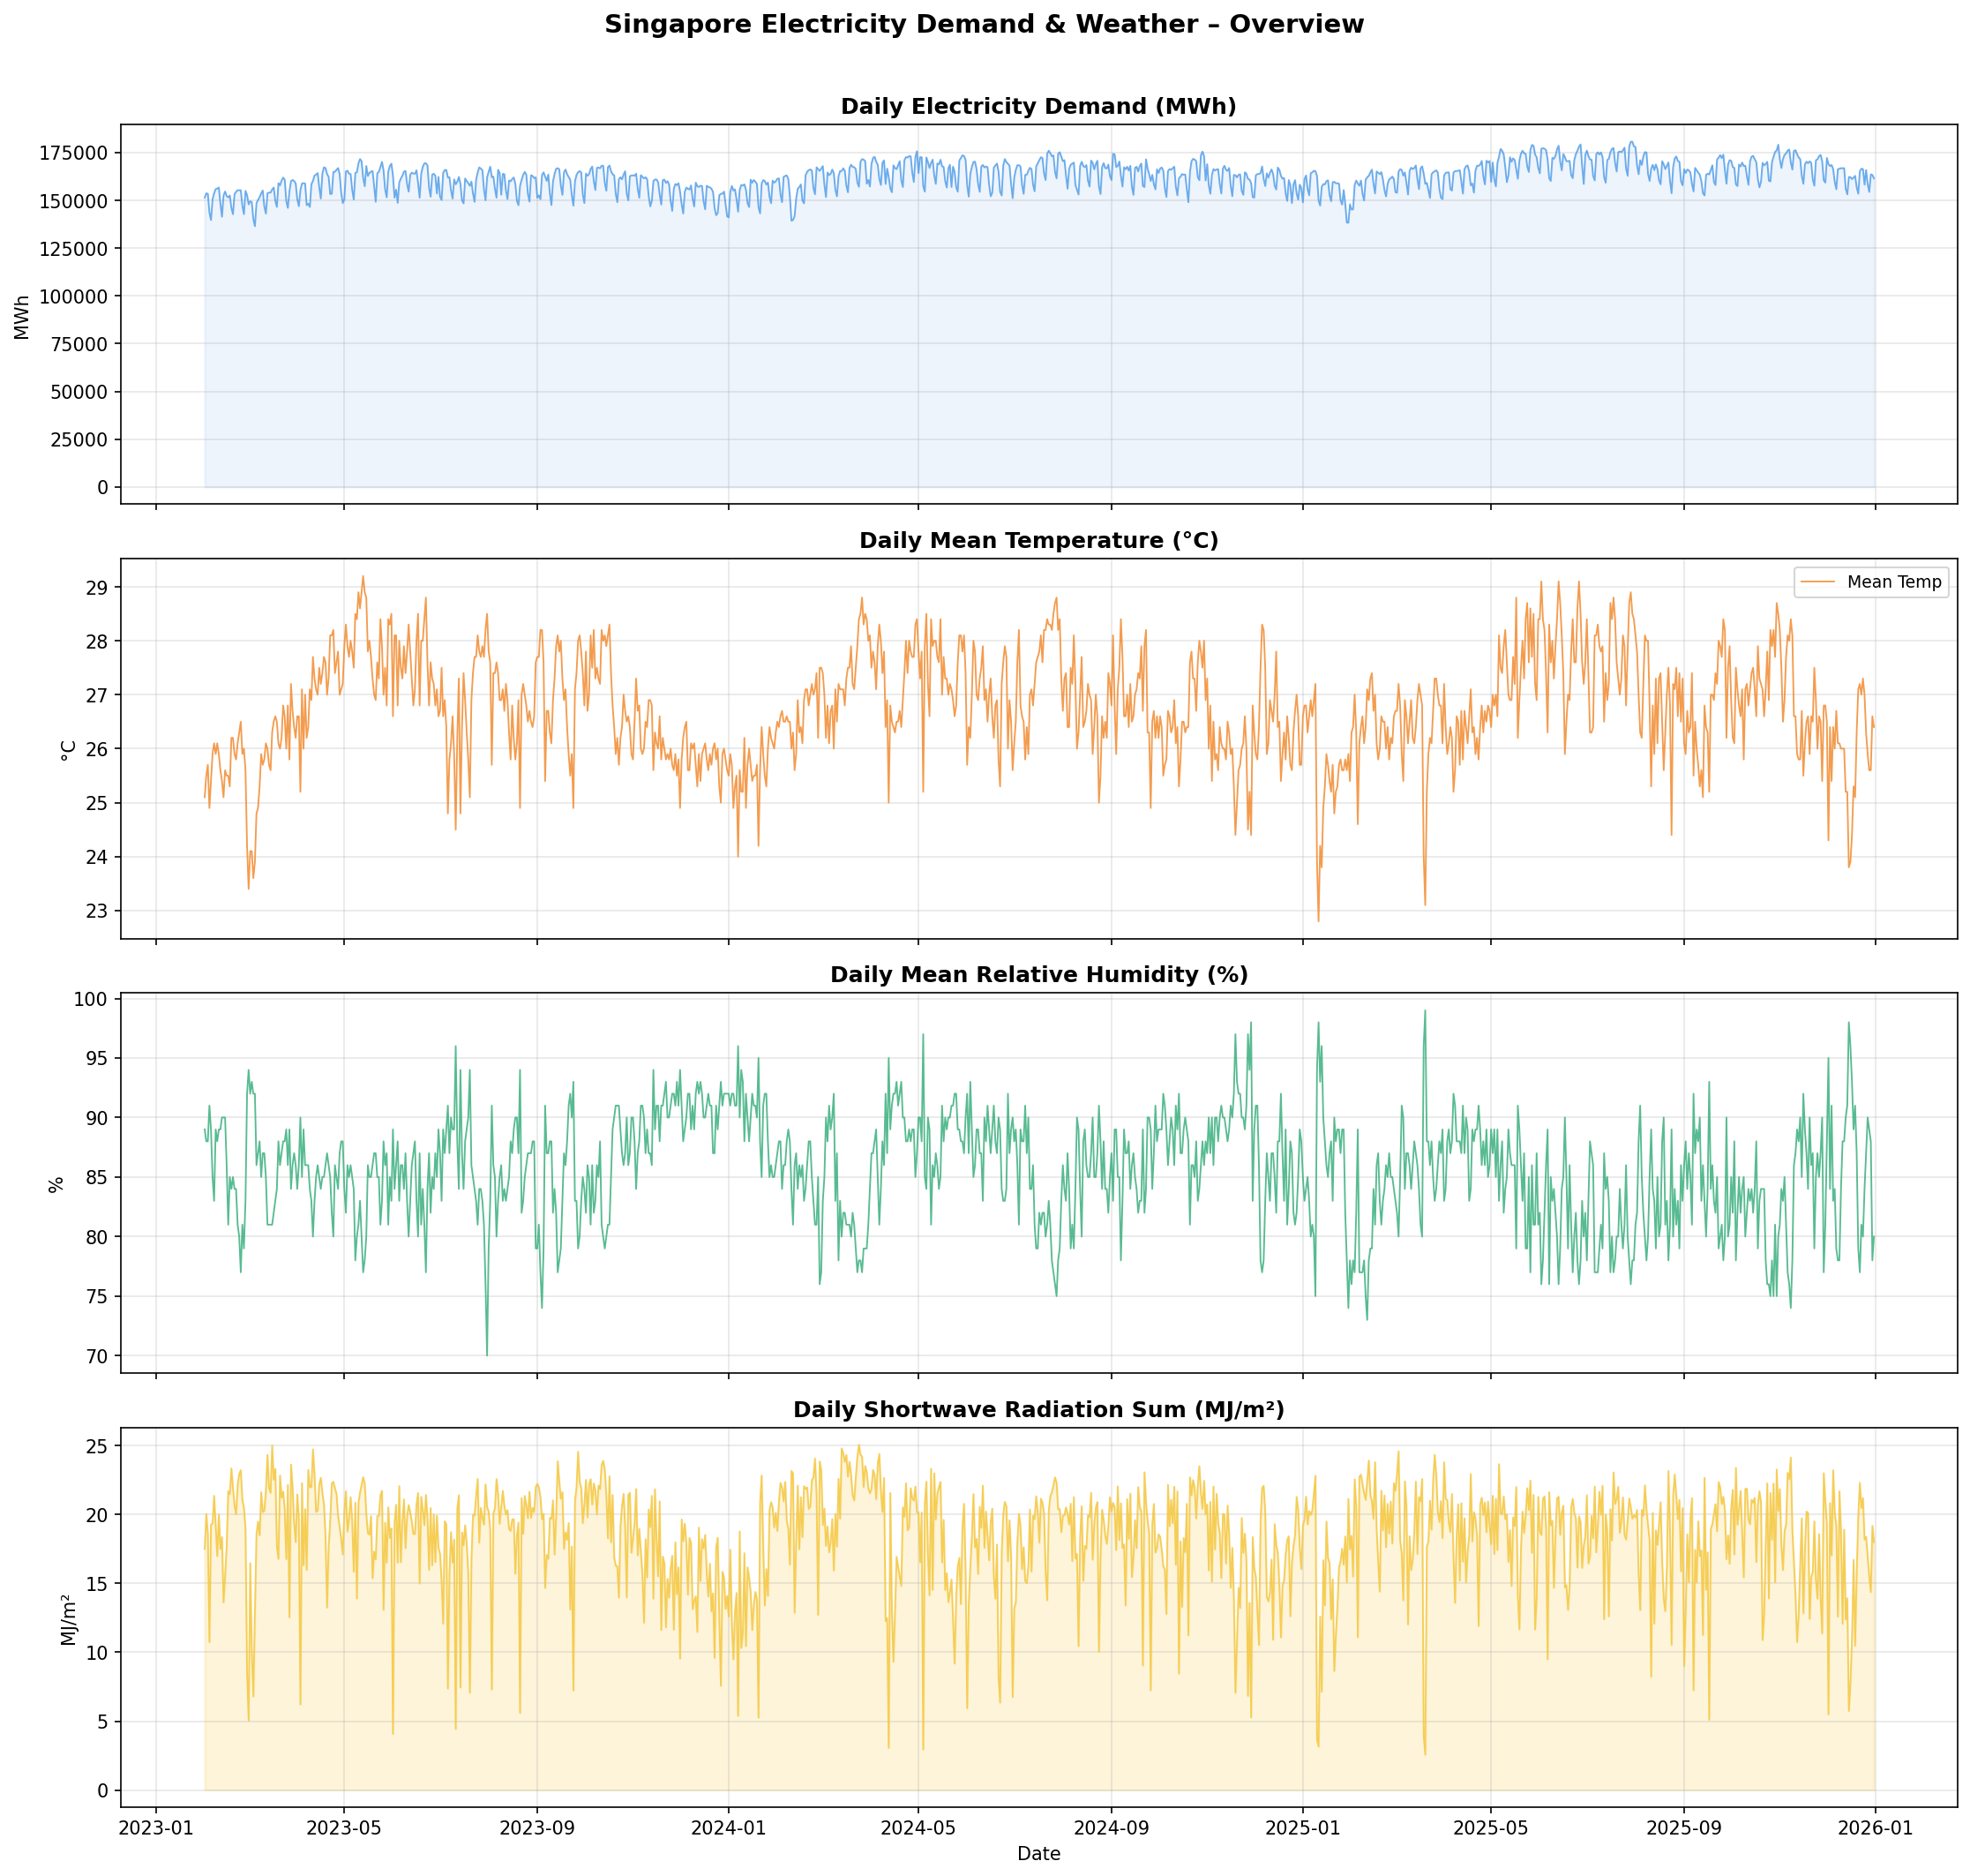
\includegraphics[width=0.92\textwidth]{design/images/eda_time_series.png}
    \caption{Daily electricity demand and weather variables in Singapore, 2023 -- 2025.}
    \label{fig:eda_timeseries}
\end{figure}

Sixteen features are constructed across four categories: \emph{weather} (the four raw variables); \emph{derived}---a Comfort Climate Index, $\mathrm{CCI} = T \times (1 + 0.01 \times H)$, which captures combined thermal stress, plus a season indicator; \emph{temporal} (day-of-week, month, weekend and Singapore public-holiday flags); and \emph{autoregressive} (demand lags at 1 and 7 days; 3- and 7-day rolling means and standard deviations). We use an 80/20 \emph{chronological} split (852 train / 213 test samples) to avoid any forward-looking bias; features are standardised only for Linear Regression.

\subsection{Models and Fair Tuning Protocol}

We compare eight configurations: a Lag-1 baseline, Linear Regression, and default Random Forest, XGBoost, and CatBoost, plus PPSO-tuned variants RF-PPSO, XGB-PPSO, and CatBoost-PPSO. The key design choice here is to give PPSO to \emph{every} tunable model under an \emph{identical} budget, rather than reserving it for CatBoost alone as Zhang et al.\ \parencite{zhang2023catboostppso} did. This way, any performance gap reflects the algorithm itself, not a tuning advantage.

We chose PPSO for three practical reasons: (i) it is essentially \emph{parameter-free}---the phasor angle automatically balances exploration and exploitation, so we avoid the circular problem of tuning the tuner; (ii) its periodic velocity modulation handles the non-convex, expensive hyperparameter landscape well, where each fitness evaluation requires multiple full model trainings; and (iii) it was already validated against six meta-heuristics in the closest prior study \parencite{zhang2023catboostppso}. For mathematical details we refer the reader to Ghasemi et al.\ \parencite{ghasemi2019ppso}.

Each model's four-dimensional search space covers its most sensitive hyperparameters (Table~\ref{tab:search_spaces}). We use a shared budget of 15 particles $\times$ 20 iterations with early stopping after 5 stagnant iterations; fitness is the mean RMSE over 3-fold \texttt{TimeSeriesSplit} cross-validation on the training set only (Figure~\ref{fig:ppso_workflow}). All seeds are fixed to 42.

\begin{table}[H]
\centering
\caption{PPSO hyperparameter search spaces (identical budget for all models).}
\label{tab:search_spaces}
\small
\begin{tabular}{@{}lllll@{}}
\toprule
\textbf{Model} & \multicolumn{4}{c}{\textbf{Tuned hyperparameters (bounds)}} \\
\midrule
Random Forest & trees (100--800) & depth (4--25) & min split (2--20) & min leaf (1--10) \\
XGBoost & trees (100--1000) & depth (3--10) & learn.\ rate (0.01--0.2) & $L_2$ (1--20) \\
CatBoost & iterations (100--800) & depth (4--10) & learn.\ rate (0.01--0.2) & $L_2$ (1--20) \\
\bottomrule
\end{tabular}
\end{table}

\begin{figure}[H]
\centering
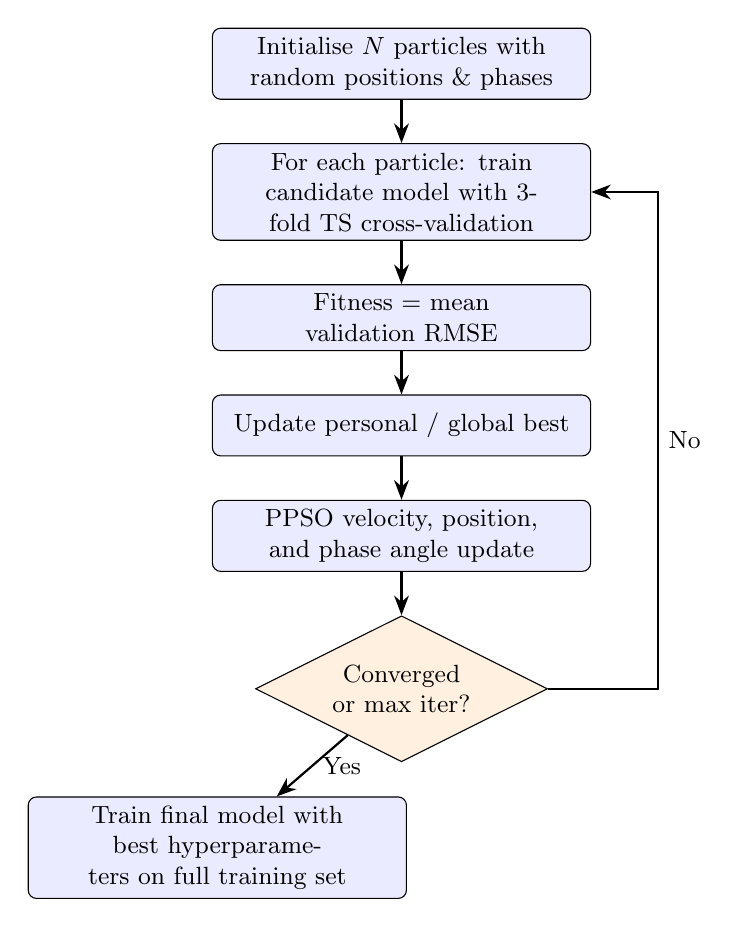
\begin{tikzpicture}[
    node distance=0.55cm,
    block/.style={rectangle, draw, fill=blue!8, text width=13em, text centered, minimum height=2.2em, rounded corners=3pt, font=\small},
    decision/.style={diamond, draw, fill=orange!12, text width=6.5em, text centered, aspect=2, inner sep=1pt, font=\small},
    arrow/.style={-{Stealth[length=2.5mm]}, thick}
]
\node[block] (init) {Initialise $N$ particles with random positions \& phases};
\node[block, below=of init] (eval) {For each particle: train candidate model with 3-fold TS cross-validation};
\node[block, below=of eval] (fitness) {Fitness = mean validation RMSE};
\node[block, below=of fitness] (update_pb) {Update personal / global best};
\node[block, below=of update_pb] (ppso_update) {PPSO velocity, position, and phase angle update};
\node[decision, below=of ppso_update] (converge) {Converged or max iter?};
\node[block, below left=0.9cm and -1cm of converge] (final) {Train final model with best hyperparameters on full training set};
\draw[arrow] (init) -- (eval);
\draw[arrow] (eval) -- (fitness);
\draw[arrow] (fitness) -- (update_pb);
\draw[arrow] (update_pb) -- (ppso_update);
\draw[arrow] (ppso_update) -- (converge);
\draw[arrow] (converge) -- node[right, font=\small]{Yes} (final);
\draw[arrow] (converge.east) -- ++(1.4,0) |- node[near start, right, font=\small]{No} (eval.east);
\end{tikzpicture}
\caption{PPSO hyperparameter optimisation workflow.}
\label{fig:ppso_workflow}
\end{figure}

\subsection{Evaluation Metrics}\label{sec:eval_metrics}

We follow Zhang et al.\ \parencite{zhang2023catboostppso} and report six metrics on the held-out test set: MAE, RMSE, MAPE, and RAE (all error-based; lower is better), plus $R^2$ and the Willmott Index (WI) \parencite{willmott1982validation} (agreement-based; higher is better). We include WI because it is more robust to outliers than $R^2$.

\subsection{Web Portal}

To make the model accessible beyond the research pipeline, we deploy it through a lightweight web portal. A FastAPI backend loads the serialised model and exposes REST endpoints on localhost (\texttt{/api/summary}, \texttt{/api/range}, \texttt{/api/predict}, \texttt{/api/forecast}), while a React/Vite frontend provides two views: a \emph{History Report} page for retrospective accuracy over a user-selected period (Figure~\ref{fig:dashboard}), and a \emph{Demand Trends} page that produces forward outlooks using live Open-Meteo weather forecasts.

\begin{figure}[H]
    \centering
    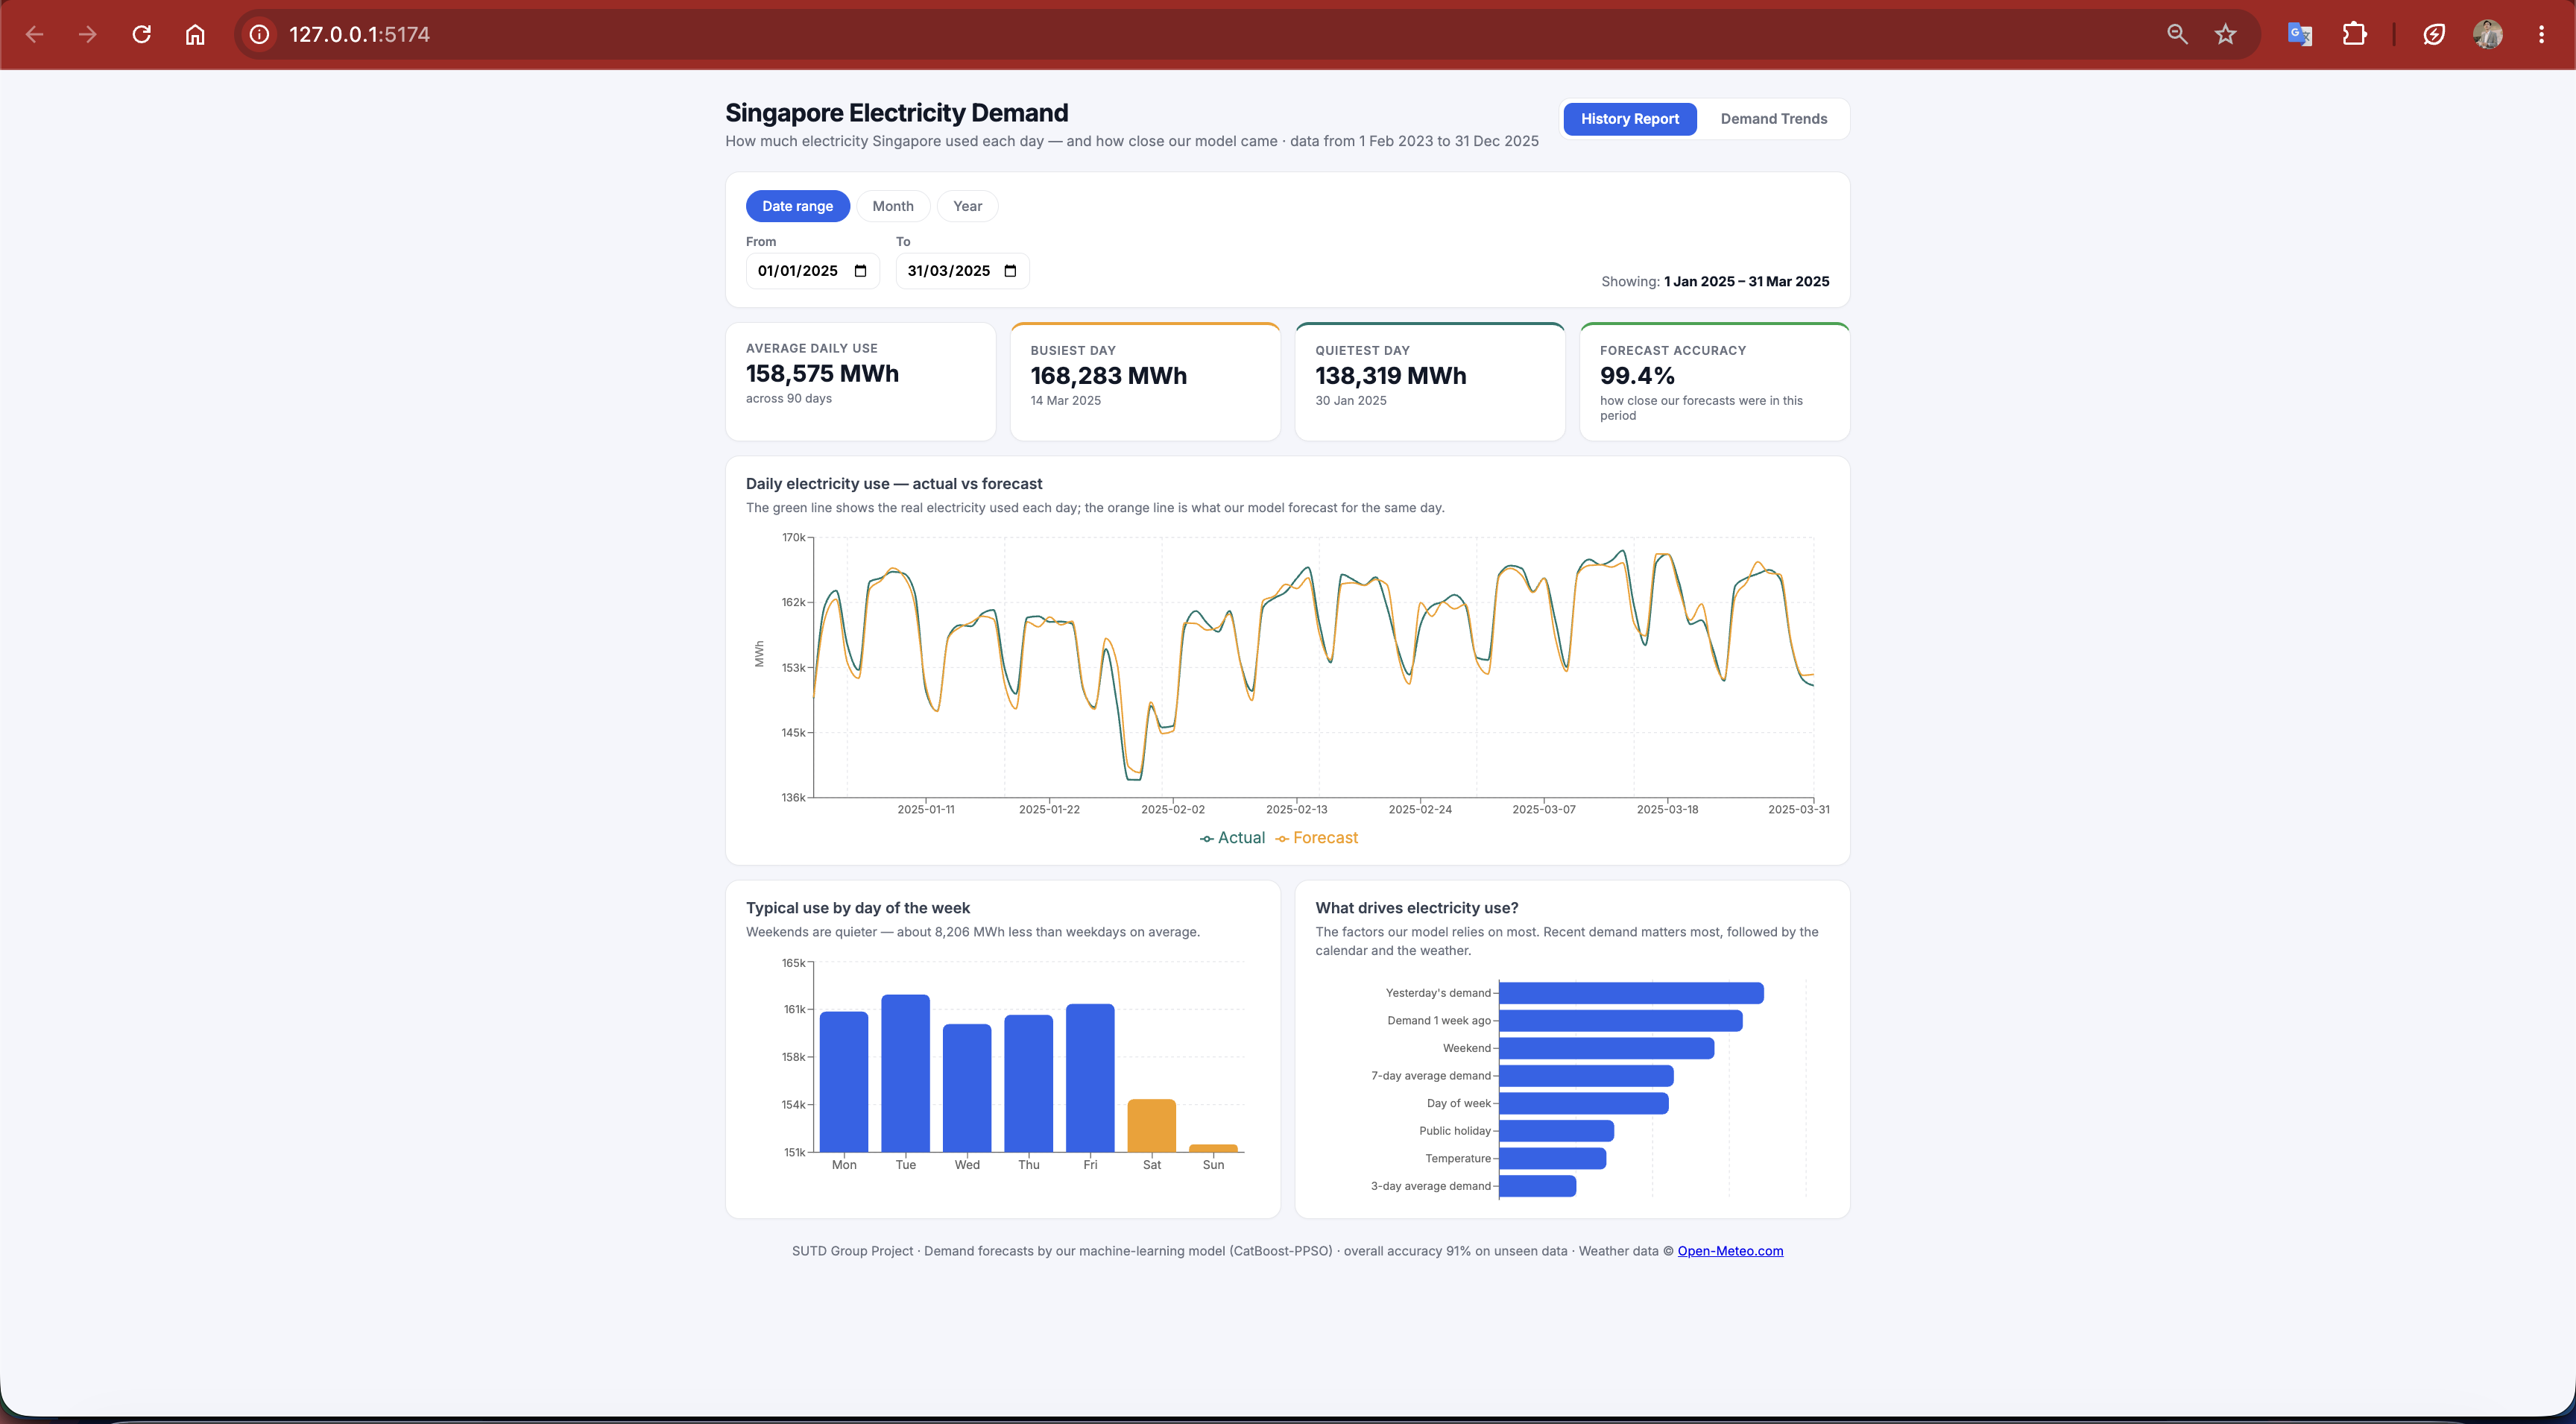
\includegraphics[width=0.88\textwidth]{impl/images/dashboard_history.png}
    \caption{History Report page of the web portal: actual vs.\ predicted demand and summary statistics for a user-selected period.}
    \label{fig:dashboard}
\end{figure}

\begin{figure}[H]
    \centering
    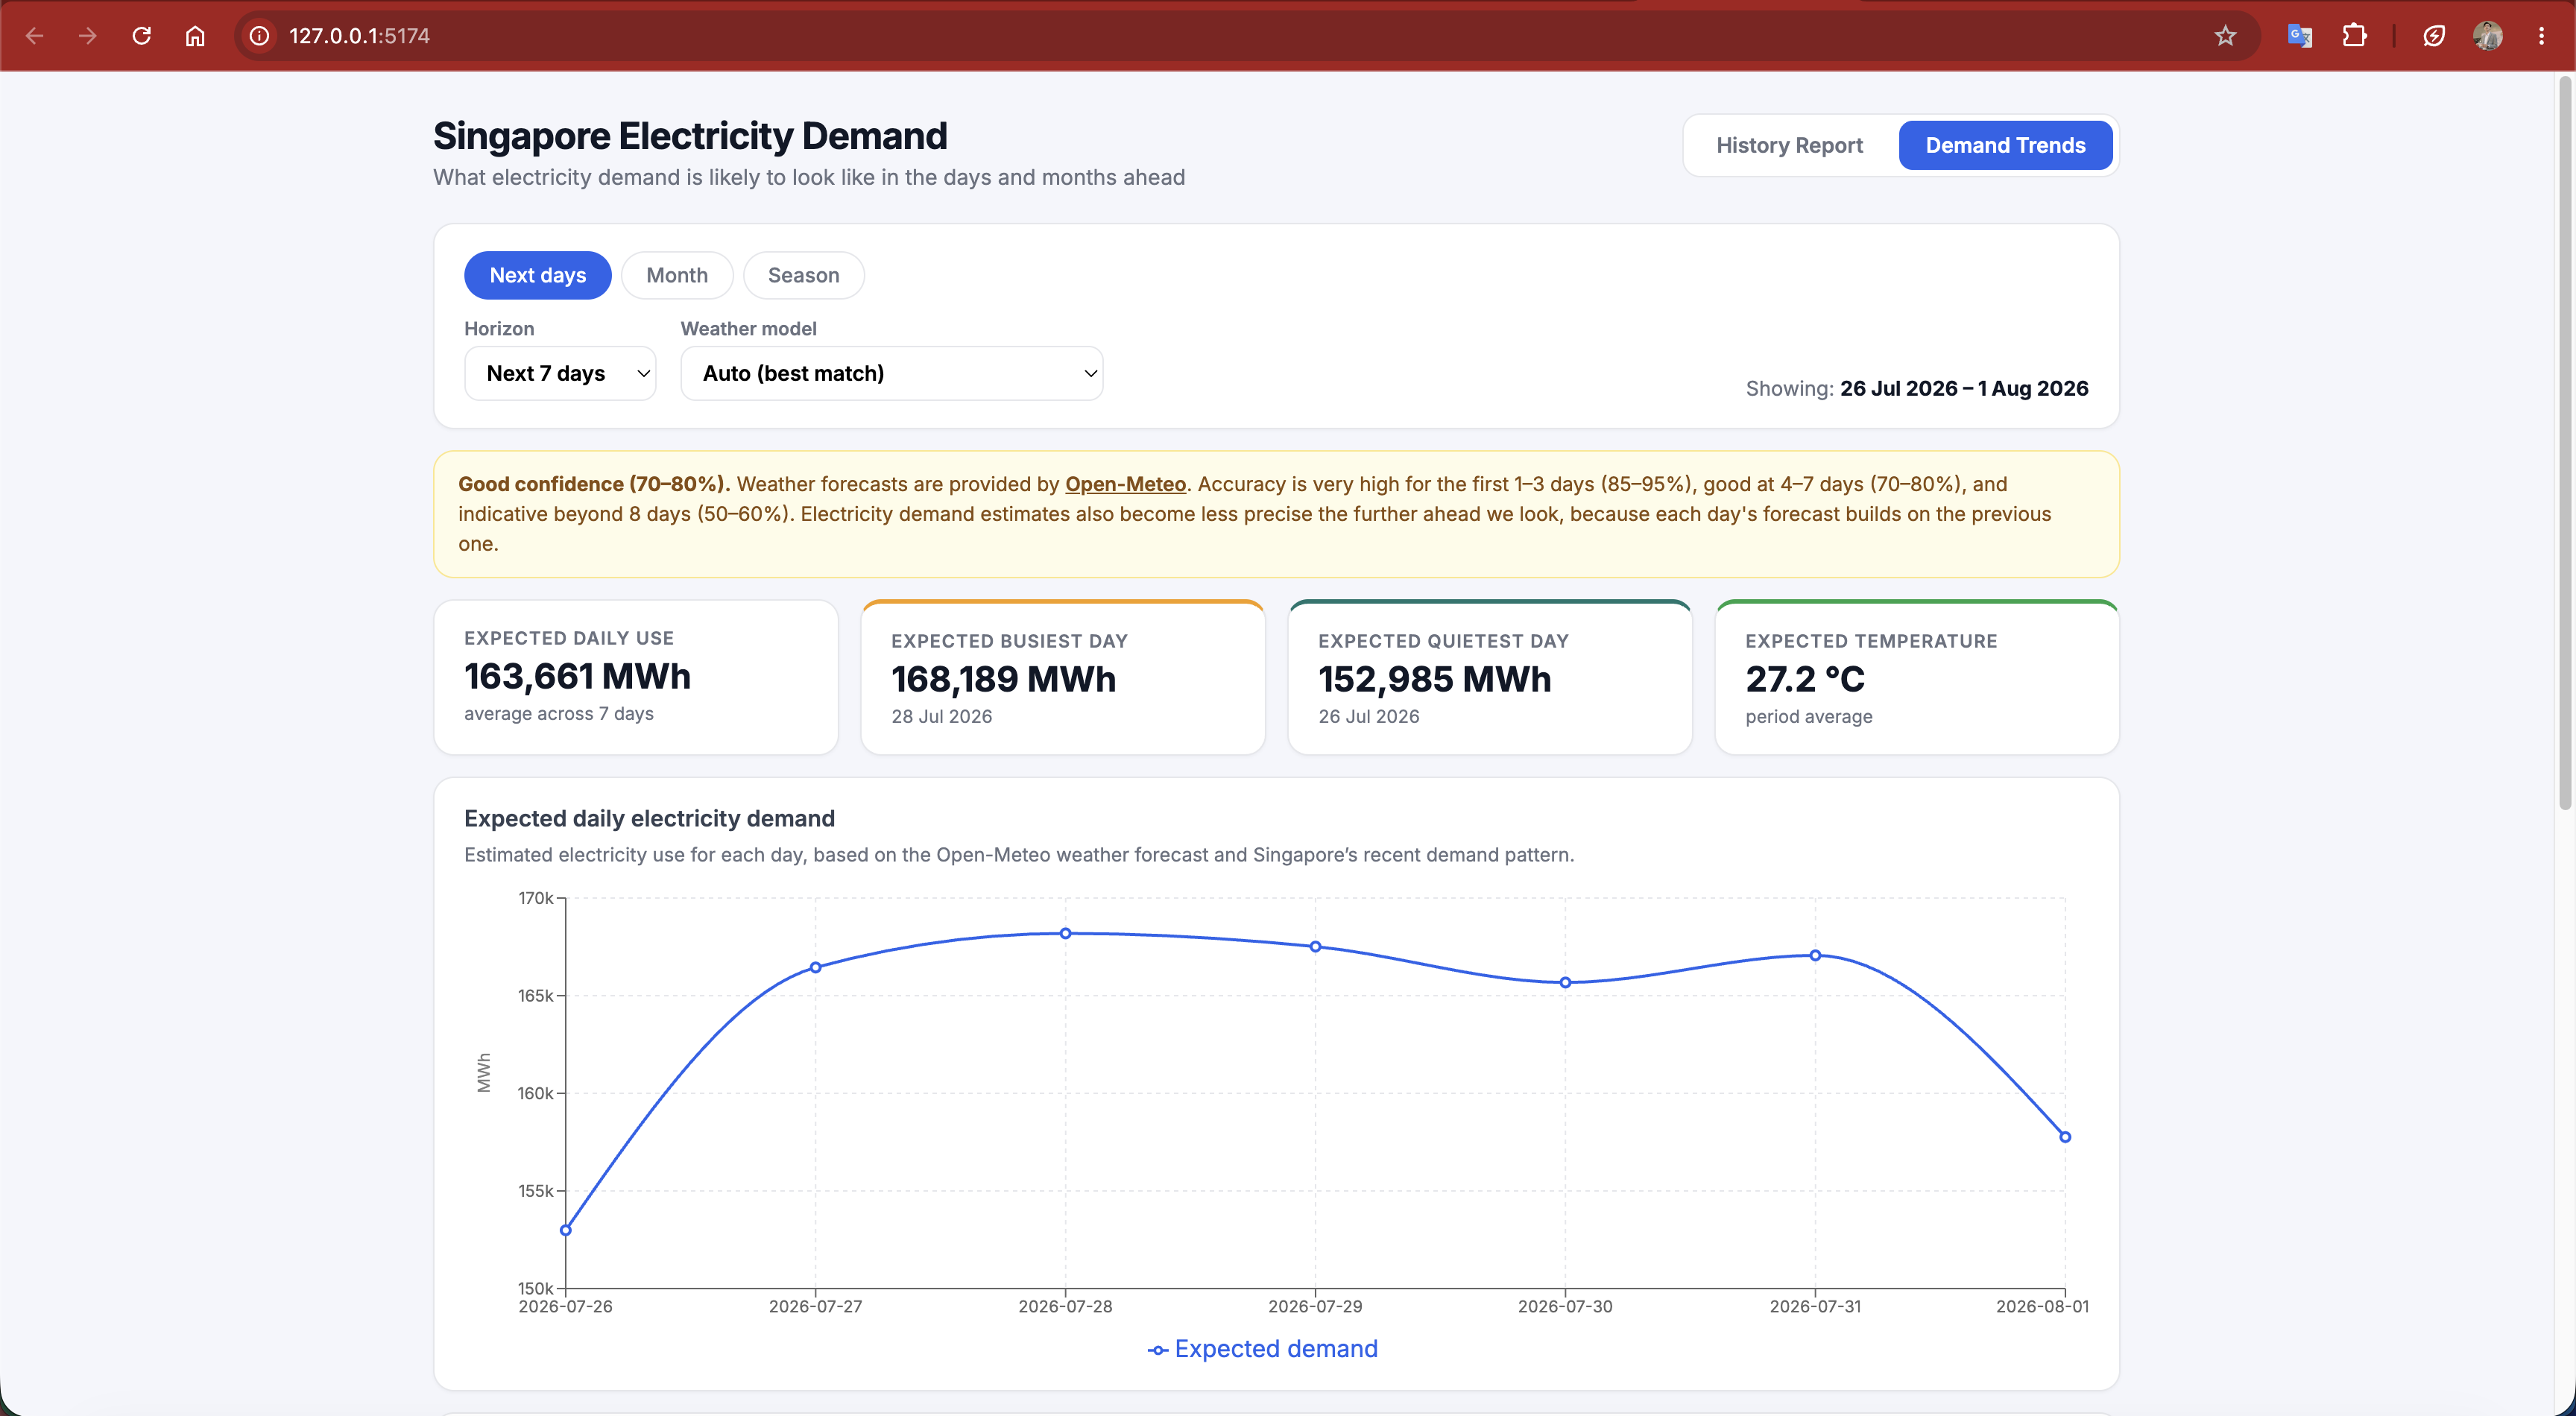
\includegraphics[width=0.88\textwidth]{impl/images/dashboard_trends.png}
    \caption{Demand Trend page of the web portal: showing the trend of electric demand through input time period.}
\end{figure}

\section{Results}\label{sec:results}

\subsection{Model Comparison}

Table~\ref{tab:model_comparison} summarises test-set performance for all eight configurations, sorted by RMSE. CatBoost-PPSO clearly separates itself from the rest, while the remaining models cluster relatively tightly---with Linear Regression, notably, sitting among the tree-based methods rather than trailing behind them.

\begin{table}[H]
\centering
\caption{Model comparison on the test set (213 samples).}
\label{tab:model_comparison}
\begin{tabular}{@{}lrrrrrr@{}}
\toprule
\textbf{Model} & \textbf{MAE} & \textbf{RMSE} & \textbf{$R^2$} & \textbf{MAPE (\%)} & \textbf{RAE} & \textbf{WI} \\
\midrule
CatBoost-PPSO & \textbf{1{,}496.2} & \textbf{1{,}895.5} & \textbf{0.9135} & \textbf{0.89} & \textbf{0.280} & \textbf{0.9774} \\
CatBoost & 1{,}679.4 & 2{,}118.8 & 0.8919 & 0.99 & 0.314 & 0.9709 \\
Linear Reg. & 1{,}693.4 & 2{,}119.2 & 0.8919 & 1.01 & 0.317 & 0.9731 \\
XGB-PPSO & 1{,}687.8 & 2{,}165.6 & 0.8871 & 1.00 & 0.315 & 0.9697 \\
Random Forest & 1{,}774.0 & 2{,}237.6 & 0.8795 & 1.05 & 0.332 & 0.9653 \\
RF-PPSO & 1{,}794.1 & 2{,}283.9 & 0.8744 & 1.06 & 0.335 & 0.9634 \\
XGBoost & 1{,}833.4 & 2{,}313.4 & 0.8712 & 1.08 & 0.343 & 0.9652 \\
\bottomrule
\end{tabular}
\end{table}

Key observations:

\begin{enumerate}
    \item \textbf{CatBoost-PPSO leads on every metric}: $R^2 = 0.914$ (over 91\% of demand variance explained), RMSE of 1{,}895.5\,MWh ($\approx$1.1\% of mean daily demand), and MAPE of 0.89\%.
    \item \textbf{PPSO gains are model-dependent.} Tuning improves CatBoost substantially (RMSE $-$10.5\%) and XGBoost moderately ($-$6.4\%), but slightly hurts Random Forest ($+$2.1\%)---likely because RF's bagging mechanism is already robust to hyperparameters, and the optimiser overfits the cross-validation folds. Since every model received the same budget, these differences confirm that CatBoost-PPSO's lead is genuine, not a by-product of preferential tuning.
    \item \textbf{Linear Regression is surprisingly competitive}, essentially tied with default CatBoost on RMSE. This tells us that the engineered autoregressive features (lag-1, rolling means) already linearise much of the problem; the value of tree models lies in capturing residual weather--calendar interactions.
    \item \textbf{All models exceed $R^2 = 0.87$ and WI $= 0.96$}, which confirms that the 16-feature set captures the dominant demand drivers regardless of model choice.
\end{enumerate}

\subsection{Prediction Behaviour}

Figure~\ref{fig:predictions} plots actual versus predicted demand for CatBoost-PPSO across the 213-day test period. The model tracks weekly cyclicity well (weekend dips are clearly reproduced), follows demand level shifts, and tends to err most on sharp holiday-related drops---events that are hard to anticipate from weather and calendar features alone.

\begin{figure}[H]
    \centering
    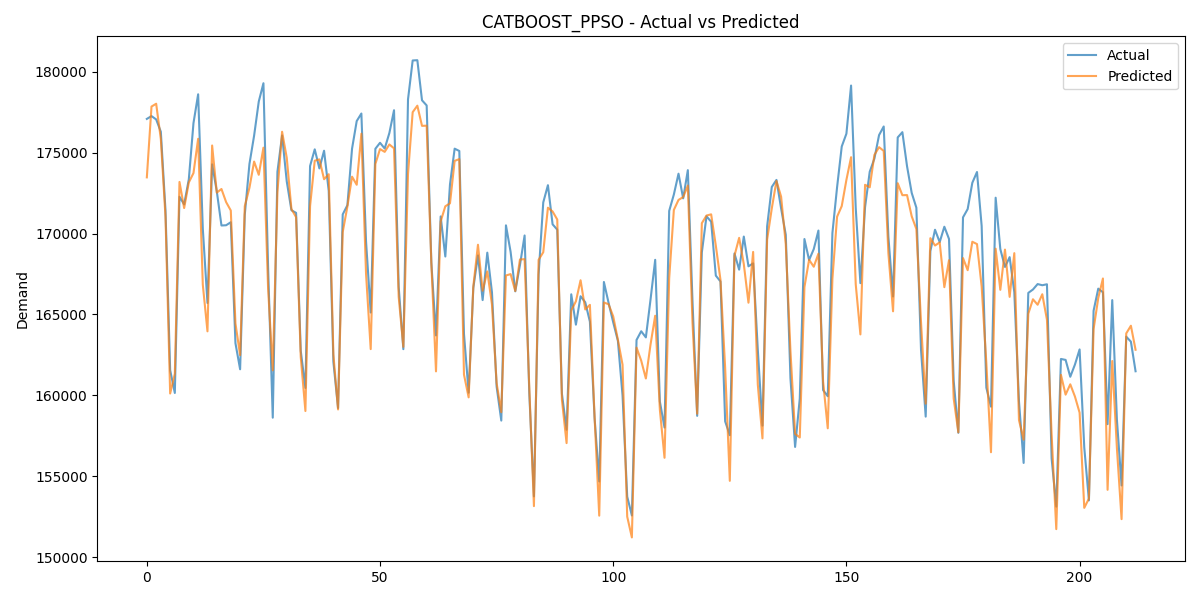
\includegraphics[width=0.88\textwidth]{eval/images/predictions_catboost_ppso.png}
    \caption{Actual vs.\ predicted daily electricity demand (MWh), CatBoost-PPSO, test set.}
    \label{fig:predictions}
\end{figure}

\subsection{Feature Importance}

Figure~\ref{fig:feature_importance} shows the CatBoost-PPSO importance scores. As expected, autoregressive features dominate---\texttt{demand\_lag\_1} and the rolling means carry the most weight---followed by \texttt{day\_of\_week}. Weather variables (temperature, humidity, CCI) sit in the mid-ranks, providing meaningful exogenous signal on top of the demand history. The same ranking holds for RF and XGBoost, suggesting this hierarchy is robust across model families.

\begin{figure}[H]
    \centering
    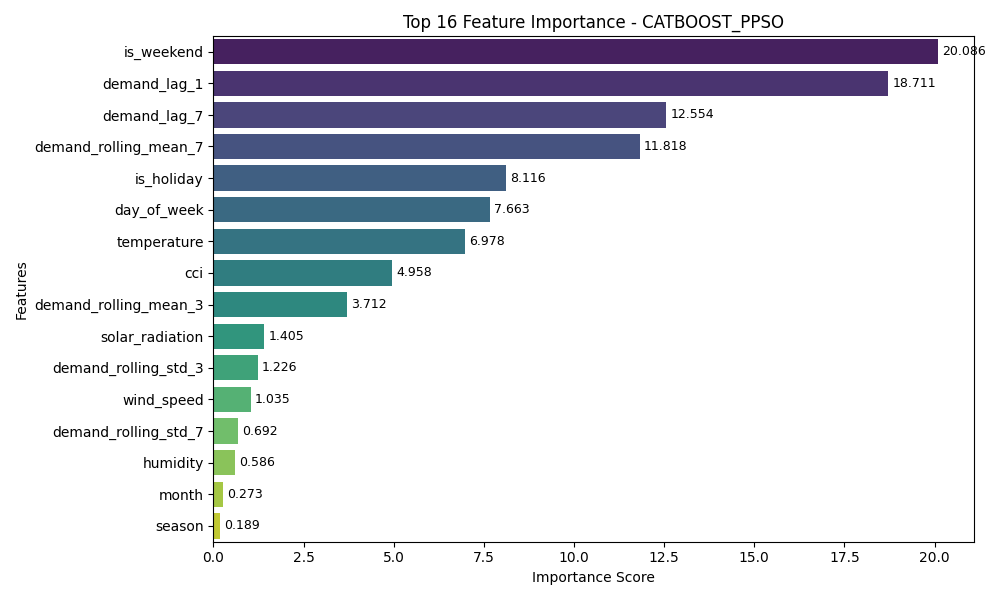
\includegraphics[width=0.78\textwidth]{eval/images/feature_importance_catboost_ppso.png}
    \caption{Feature importance, CatBoost-PPSO. Autoregressive features dominate, with weather variables providing secondary signal.}
    \label{fig:feature_importance}
\end{figure}

\subsection{Impact of PPSO Optimisation}

To isolate the tuning effect, Table~\ref{tab:ppso_impact} breaks down the before-and-after metrics for CatBoost, the model that benefited most.

\begin{table}[H]
\centering
\caption{Impact of PPSO hyperparameter optimisation on CatBoost.}
\label{tab:ppso_impact}
\begin{tabular}{@{}lrrr@{}}
\toprule
\textbf{Metric} & \textbf{CatBoost (default)} & \textbf{CatBoost-PPSO} & \textbf{Improvement} \\
\midrule
MAE (MWh) & 1{,}679.4 & 1{,}496.2 & $-$10.9\% \\
RMSE (MWh) & 2{,}118.8 & 1{,}895.5 & $-$10.5\% \\
$R^2$ & 0.8919 & 0.9135 & $+$2.2 pp \\
MAPE (\%) & 0.99 & 0.89 & $-$10.6\% \\
RAE & 0.314 & 0.280 & $-$10.9\% \\
WI & 0.971 & 0.977 & $+$0.6 pp \\
\bottomrule
\end{tabular}
\end{table}

Compared with Zhang et al.\ \parencite{zhang2023catboostppso}, who reported $R^2 = 0.971$ on hourly single-customer data, our lower $R^2$ (0.914) is not surprising: daily national demand aggregates consumption across millions of heterogeneous users, which inevitably adds unexplained variance. Still, the fact that the methodology transfers across such different scales, resolutions, and climates is encouraging.

\section{Discussion}\label{sec:discussion}

\subsection{Interpretation}
Beyond the raw rankings, three findings stand out. First, hyperparameter optimisation is not a universal win. PPSO helped the two gradient-boosted models, whose accuracy depends heavily on learning rate and regularisation strength, but it actually hurt Random Forest. This makes sense: RF's bagging mechanism is inherently stable across a wide range of hyperparameters, so an aggressive search is more likely to overfit the cross-validation folds than to find a genuinely better configuration. Had we only tuned CatBoost---as is common in the literature---this distinction would have been invisible, and the reported gains could easily be mistaken for algorithmic superiority rather than a tuning artefact.

Second, the strong showing of Linear Regression tells us something important about the problem structure. Once we include lag-1 demand and rolling statistics, most of the daily signal is already captured linearly. The non-linear models earn their keep on the residual: weather--calendar interactions (e.g.\ a hot weekday versus a cool public holiday) that a linear model cannot represent. CatBoost's native categorical handling is especially well-suited here, which helps explain why it pulls ahead of XGBoost and RF once PPSO finds good hyperparameters.

Third, using time-series cross-validation inside the PPSO fitness function turned out to be essential. Early experiments with random K-fold produced optimistic fitness values that did not hold up on the test period. Respecting temporal order in every evaluation step---from the train/test split down to the inner CV folds---was critical for honest results.

\subsection{Limitations}
Several limitations should be kept in mind. Daily aggregation hides intra-day peaks; Open-Meteo reanalysis data may differ from ground-station measurements; external shocks such as economic events or policy changes are not modelled; PPSO is stochastic and our results reflect a single seeded run; and multi-day portal forecasts inherit whatever error exists in the upstream weather forecast.

\subsection{Future work}
Moving to hourly resolution with intra-day features would be the most impactful next step. We would also like to run multi-seed PPSO experiments with statistical significance testing, benchmark sequence models (LSTM, Transformer) under the same fair-tuning protocol, and add online retraining to the deployed portal so the model stays current as demand patterns evolve.

\section{Conclusion}\label{sec:conclusion}

We built an end-to-end pipeline for daily electricity demand forecasting in Singapore, training and comparing eight model configurations on a 16-feature dataset covering weather, calendar, and autoregressive variables from February 2023 to December 2025. Our main takeaways are:

\begin{enumerate}
    \item \textbf{CatBoost-PPSO is the strongest model}, with $R^2 = 0.914$, MAE of 1{,}496.2\,MWh, RMSE of 1{,}895.5\,MWh, and MAPE of 0.89\% on the held-out test set.
    \item \textbf{Fair tuning matters.} Giving every tree model the same PPSO budget revealed that the gain is large for CatBoost ($-$10.5\% RMSE), moderate for XGBoost ($-$6.4\%), and absent for Random Forest. This means CatBoost-PPSO's lead comes from the algorithm itself, not from receiving preferential optimisation.
    \item \textbf{Autoregressive features carry most of the signal}; weather variables (temperature, humidity, CCI) add meaningful secondary information, consistent with Singapore's cooling-driven demand profile.
    \item \textbf{The approach generalises}: CatBoost-PPSO, originally validated on hourly single-customer data \parencite{zhang2023catboostppso}, transfers well to daily national-level demand in an equatorial climate.
    \item \textbf{From pipeline to product}: we deployed the best model in a web portal that offers retrospective accuracy reports and weather-driven demand outlooks, showing a viable path from research code to a decision-support tool for grid operators and energy planners.
\end{enumerate}


\footnotesize
\printbibliography
\normalsize

\end{document}
